\documentclass[11pt]{article}
\usepackage[margin=1in]{geometry}
\usepackage{amsmath,amssymb,booktabs,authblk,graphicx,url}
\newcommand{\grad}{\nabla}
\newcommand{\half}{\tfrac12}

\title{RealQM on Conduction}
\author[1]{Claes Johnson}
\affil[1]{KTH Royal Institute of Technology, SE-100 44 Stockholm, Sweden \\
\texttt{claesjohnson@gmail.com}}
\date{}

\begin{document}
\maketitle

\begin{abstract}
\noindent RealQM, as an alternative to textbook quantum mechanics, represents an $N$-electron system
by $N$ real-valued wave functions $\psi_i(x)$, with $x$ a coordinate in
three-dimensional Euclidean space, whose squares $\psi_i^2$ are unit charge densities with
non-overlapping supports meeting at free interfaces. The physics is carried by a single energy
functional: electron Coulomb potential energy without self-repulsion, plus kinetic energy. No other
force enters it and nothing in it is fitted. The ground state is the configuration minimising that
functional over the supports as well as over the wave functions, so the interfaces are unknowns of
the problem rather than inputs to it. The cost of that minimisation scales as $N$ times the number of mesh points.

RealQM has already been applied to solids --- ionic crystals under melting and under shear,
molecular solids including ice and solid nitrogen, a lithium lattice of a hundred atoms recovering
from a perturbation under its own dynamics --- and, further afield, to molecular binding, hydrogen
bonds and solvation, to ionisation energies across the periodic table, and to nuclear binding by
dual Coulomb confinement. All of it is \emph{bound} matter, where an attractor is present and the
charge is where the attractor is, and in none of it was transport attempted.

The task posed here is conduction, the first question asked of RealQM about charge that no
attractor holds in place: the cost of advancing the electron pattern of a solid by one lattice site,
which is the activation energy for charge transport. The answer is obtained from Coulomb interaction and kinetic energy
alone. The geometry is here specified rather than found: the supports are held
while the wave functions relax, so what is computed is a constrained minimum, and the arrangements held
are of the kind this framework settles into when its boundaries are free --- the constraint selects
a coordinate along which to displace the charge, and does not invent the configuration. No such
computation appears to have been carried out before. The
reason is structural rather than a want of effort. In textbook quantum mechanics the $N$-electron
state is a function on a $3N$-dimensional configuration space, which on a grid costs that grid
raised to the power $N$ and is beyond computation for any $N$ of interest, so every route that can actually be followed first reduces the dimension and then
repairs the reduction with modelled parameters --- a relaxation time, a transfer integral, an
effective mass --- and the transport energy comes out of those parameters rather than out of the
two terms it is made of. Working in three dimensions from
the start removes the need for them, at a cost linear in $N$ rather than exponential in it. That is
the new capability reported here: the quantity is computed rather than modelled.

Computationally the difficulty is one of scale. Atomic energies are tens of electron-volts,
semiconductor activation is $50$--$500$~meV per carrier and metallic conduction sets in near
$20$~meV, while the total energy of a chain long enough to pose the question is thousands of
electron-volts. The barrier sought is therefore between $10^{-3}$ and $10^{-5}$ of the number a calculation
returns, depending on the arrangement.
It is not reached by computing that number to five figures, but by differencing two configurations
of the same system --- the same electrons, the same kernels, the same grid, differing only in where
a few interior domain walls sit --- so that every large contribution to the error is common to both
and cancels.

Four cases are computed --- three arrangements of charge and one of them again with its carriers
stiffened. Three of them yield a barrier to advancing the electron pattern by one site, and it
differs by a factor of twenty between them; the fourth yields none, its landscape having no minimum
at the registry a barrier would be measured from. None is a one-dimensional model. The wave functions are functions
on ordinary three-dimensional space, the domains are regions of it, and the calculations run on
grids of some two to three million points; in three of the cases what is arranged along a line is
the nuclei, and in the fourth they sit on a simple cubic lattice. A \textbf{chain of hydrogen atoms},
one electron to each kernel, gives ${\approx}394$~meV per electron and a polarisability
$\alpha=7.6N$, extensive in the number of electrons. Its landscape is not the assumed one: scanned
across a period, the minimum lies not at registry but near a quarter spacing, $196$~meV below the
arrangement with each electron centred on its own kernel, and the two maxima are of unequal height,
so advancing one site is a two-step passage rather than a single crossing. A \textbf{cable of Li ions}, the carriers
standing off closed cores, gives ${\approx}246$~meV. A \textbf{simple cubic lattice} of $72$ hydrogen atoms, three by three
by eight at the same spacing in all three directions, yields no barrier: windowed and scanned, its
landscape descends away from registry --- $997$~meV per carrier below it at a three-eighths
displacement --- so registry is not its minimum and the quantity a global difference would return is
not a barrier at all. It is reported for what it does settle --- it makes the nuclei a crystal
rather than a line, so the carrier density becomes a property of the structure instead of a
convention; it is the best-conditioned calculation here; and it shows the assumed registry failing a
second time, in three dimensions. The first two are the computed values, at the coefficient
$\half$ that the kinetic term carries throughout. Varying that coefficient is then a sensitivity and
not a result: raised to $0.75$ the cable's barrier is $66$~meV, at $0.9$ it is $20$~meV --- below
room temperature's $kT=26$~meV, so a cable so stiffened would not hold its charge --- and at $1.0$
it is $1$~meV. No value was sought that reproduces anything measured, and the third arrangement is
reported to show how soft the barrier is in this one coefficient, not to exhibit a conductor. The
preferred registry, carriers on their own ion sites, is unchanged across the range, so what the
stiffening weakens is the pinning itself and not merely its location.

What is computed is an energetics of charge, and one transport quantity follows from it with
nothing added. A uniform field tilts the landscape and nothing more, so the field at which the
barrier disappears is a property of $E(d)$ alone: $5.2\times10^{9}$, $3.2\times10^{9}$ and
$2.6\times10^{8}$~V\,m$^{-1}$ for the chain, the cable and the stiffened cable. The first two are above the dielectric
strength of silica and would break down before they would slide; the stiffened cable is below it and
would slide first.

A conductivity requires more, and the division is the ordinary one: an energy landscape from a
theory of charge, a rate from a theory of statistics laid over it, as density functional theory is
routinely used with transition-state theory. In the activated regime two things must be supplied, a clock and a
temperature, and with them the drift velocity follows from the landscape directly. Only the
temperature is an import the framework could not in principle replace, a frequency being available
from nuclei that already move classically. Taken on those terms the barriers give room-temperature conductivities of
$0.1$ and $10$~S\,m$^{-1}$, which bracket intrinsic germanium at $2$~S\,m$^{-1}$. The attempt
frequencies come out at $h\nu=76$ and $23$~meV, lattice energies that were not asked for and a check
that the mass entering them is of the right kind; but they are computed from the curvature a
sinusoid would have, and the scan shows the real well to be much flatter than that, so both
frequencies --- and the conductivities with them --- are overestimates by a factor this article does
not fix. The barriers are
upper bounds for a reason independent of mechanism --- a barrier is a minimum over paths joining two
registries and the rigid slide is one such path --- so the conductivities are lower bounds by a
factor this article does not determine.
\end{abstract}

\section{The basic question posed to RealQM}

RealQM represents an $N$-electron system in terms of $N$ real-valued wave functions $\psi_i(x)$,
with $x$ a coordinate in three-dimensional Euclidean space, whose squares $\psi_i^2$ are unit charge
densities with non-overlapping supports $\Omega_i$ meeting at free interfaces. The physics of the system is described through its energy functional, the sum of
electron Coulomb potential energy without self-repulsion and kinetic energy, with no other force entering and nothing fitted. Explicitly,
\begin{equation}\label{eq:E}
E[\{\psi_i\},\{\Omega_i\}]=\sum_i\int_{\Omega_i}\Bigl(\half|\grad\psi_i|^2
-\sum_s\frac{Z_s}{|x-x_s|}\psi_i^2\Bigr)dx
+\half\sum_{i\neq j}\iint\frac{\psi_i^2(x)\psi_j^2(y)}{|x-y|}\,dx\,dy,
\end{equation}
where $i$ and $j$ index the electrons, $s$ indexes the nuclei, $Z_s$ and $x_s$ are the charge and
position of nucleus $s$, and $y$ is a second space coordinate; the supports are disjoint and
$\int_{\Omega_i}\psi_i^2=1$. Atomic
units are used throughout: lengths in Bohr radii $a_0=0.529$~\AA, energies in hartree,
$1$~Ha${}=27.211$~eV.

The ground state of the system is the configuration minimising this energy, the minimisation running
over the supports as well as over the wave functions, so that the interfaces are unknowns of the
problem and not inputs to it; excited states are the other stationary points of the same energy. The
cost of minimising \eqref{eq:E} is the cost of $N$ Poisson problems on the grid. The potential of the
whole electron distribution is a single solve; but the double sum in \eqref{eq:E} omits $i=j$, so
what each electron must be given is the potential of all the \emph{others} --- the total less its own
field --- and its own field is a different function for every $i$. A multigrid solve costs work
proportional to the number of mesh points, so a relaxation step performs $N$ times the mesh of
arithmetic. The single wave function of textbook quantum mechanics, by contrast, lives on a $3N$-dimensional
configuration space and costs one grid raised to the power $N$. Linear against
exponential is the difference between a calculation that can be run and one that cannot, and it is
why \S8 can put seventy-two atoms on a lattice with no change of method and no loss of accuracy ---
indeed with the smallest residual in this article --- and why the lithium lattice cited below runs
at a hundred atoms. That is the framework. The
calculations reported here do not use it in full: they specify the supports and hold them, for the
reasons \S3 gives, so what is computed is a constrained minimum over the wave functions at a stated
partition.

Every previous application of RealQM --- solids, among them ionic crystals under melting and shear
and a lithium lattice of a hundred atoms under its own dynamics \cite{code}; molecular binding,
hydrogen bonds and solvation \cite{realqm,realqmbook}; ionisation energies across the periodic table
\cite{realatoms}; nuclear binding by dual Coulomb confinement \cite{realnucleus} --- has been to
\emph{bound} matter, where an attractor is always present and the charge is where the attractor is.
Conduction is the first question that asks about charge which is not where an attractor holds it, and
the framework has no separate machinery for it: the same energy, the same domains, in a different
arrangement of the same two kinds of charge.

The task posed to it here is accordingly this: what does it cost to advance the electron pattern of
a solid by one lattice site, which is the activation energy for charge transport. What enters the
answer is the two terms of \eqref{eq:E} and a specification of the nuclei, with nothing adjusted to
reproduce a measured quantity, and such a computation does not appear to have been carried out
before, for reasons \S2 sets out.

What is computed is the energetics, and the limit of that is best put dimensionally: a minimisation
of \eqref{eq:E} yields energies, while a current is charge per time and a conductivity is charge per
time per field. No quantity of energy supplies a time. So a rate theory must be brought in from
outside, here as everywhere else, and \S7 is exact about which parts of that import the framework
might one day supply for itself --- the time scale being the part that a lattice already moving
classically could provide.

\paragraph{Three-dimensional throughout.} Most of the arrangements below place their nuclei on a
line --- the exception is the cubic lattice of \S8 --- and it is worth saying at once that nothing
else about them is one-dimensional. Each $\psi_i$ is
a function on $\mathbb{R}^3$, each support $\Omega_i$ is a region of it with a two-dimensional
free surface, and the domains tile a three-dimensional box --- $138^3$ and $148^3$ points for
the two box sizes used here. A linear chain of nuclei is the smallest arrangement in which a registry
between a carrier lattice and an ion lattice can be posed at all, which is why it is used; it is
not a reduction of the electronic problem, and there is no step anywhere in this article at
which a dimension is integrated out.

\paragraph{The arrangements, and what they are made of.} The first is a \textbf{chain of atoms}:
one kernel per site with its valence electron occupying the same region, which is what a hydrogen
chain is and what an alkali is to a first approximation. The second is a \textbf{cable of ions
surrounded by electrons}: kernels screened by their own core electrons, with the valence charge
standing off outside them, which is how a wire is built. The third, in \S8, is a \textbf{simple cubic
lattice} of the first: the same spacing in all three directions, three chains by three by eight
sites, so the slide runs along the long axis of the sample.

What each is made of should be stated precisely, since the sense in which they are real matters and
the sense in which they are not is dealt with in \S2. Each is specified by nuclear charges and
positions and by how many electrons sit at each site, and nothing else: the interactions are
Coulomb, the kinetic term is the one in \eqref{eq:E}, and no quantity stands in for an electron or
for a potential. There is no pseudopotential in any of them, no hopping parameter, no on-site
repulsion $U$, no uniform background, no band. They are in that sense not lattice models but
assemblies of nuclei and electrons. What they are not is arrangements anyone has measured, which
\S2 sets out.

\section{What textbook quantum mechanics offers}

Recall that textbook quantum mechanics is based on Schr\"odinger's equation in $3N$ dimensions for a
single antisymmetric wave function $\Psi(x_1,\dots,x_N)$, with the exclusion principle carried by the
antisymmetry and with a Hamiltonian built, like \eqref{eq:E}, from Coulomb interaction and kinetic
energy alone.
But the cost of solving it is exponential in $N$, and the models actually used --- Hartree,
Kohn--Sham and their descendants --- always include drastic reductions of the dimensionality. There
is thus no textbook treatment of conduction and insulation based on Schr\"odinger's equation. There
is a stack of models, each carrying quantities supplied from measurement.

Metal is separated from insulator by a gap at the Fermi level \cite{ashcroft}, and in practice the gap comes from a chosen exchange--correlation
functional \cite{kohnsham}; the Kohn--Sham gap is not the excitation gap even for the exact
functional \cite{perdewlevy}, and the discrepancy is repaired by hybrid mixing or a $GW$ self-energy
\cite{hedin}. Transport is then a second model on top of the first: a Boltzmann equation closed by a
relaxation time, with an effective mass and a deformation potential for the semiconductor
\cite{bardeen}; a transfer integral and a reorganisation energy for a hopping conductor
\cite{marcus,holstein}; a localisation length and a density of states at the Fermi level for
variable-range hopping in a disordered one \cite{mott}; a Hubbard $U$ where the band picture fails
outright and the material insulates by correlation instead \cite{hubbard,imada}. The recent direction of travel is worth noting, because it runs the other way: learned
exchange--correlation functionals \cite{dm21} replace a handful of constructed parameters with a
neural network trained on reference data, and interatomic potentials fitted to density-functional
output \cite{mace} dispense with the functional altogether in favour of a model fitted end to end.
These are effective, and the neural wavefunction methods \cite{ferminet} are a genuine advance on
the variational problem --- but they solve the $3N$-dimensional problem with a better ansatz, and
the density-functional line answers the cost of that problem by adding fitted content rather than
removing it.

The point of the contrast is not performance. These are the methods in practical use, calibrated
against measured data, and this article makes no claim about how they perform. It is that they are
several models with parameters, addressing the regimes separately, whereas what follows is one
energy with none, in which the regimes differ by how the charge is arranged.

\paragraph{How the comparison should be read.} Two misreadings are worth heading off, because they
pull in opposite directions. The first is to score RealQM against the calibrated performance of
methods that carry fitted quantities. That is the wrong axis: the claim here concerns what the model
contains, not whether it beats a percentage. Nothing in \eqref{eq:E} is adjusted to reproduce a transport
quantity --- the sensitivity of \S6 varies the kinetic coefficient to ask how much the answer turns
on it, and takes no value from any measurement --- and a framework carrying no fitted transport
content should not be judged by the calibrated performance of ones that do. The two are different
claims: a fitted method reproducing measured data establishes that its parameters transfer, which is
a statement about the fit; an unfitted one doing so is a statement about the formulation.

The second is to require agreement with a near-exact solution of Schr\"odinger's equation ---
configuration interaction, coupled cluster, quantum Monte Carlo --- for the same system. RealQM is
not an approximation to that equation. It is a different formulation, and it is not empirically
equivalent to it: the two make different predictions, and where they differ the question is which
the world agrees with, not which reproduces the other. Disagreement with a benchmark solution of the
$3N$-dimensional problem is therefore not a defect in a formulation that does not claim to solve it.

What remains, and it is the only thing that adjudicates, is measurement. RealQM's record there is on
bound matter, and it is mixed, which is worth stating rather than summarising favourably. The
binding of H$_2$ comes out $4.20$~eV against $4.75$ measured. Atomic total energies across the first
three periods are reproduced to about $1.7$ per cent without fitting, but the \emph{ionisation}
energies derived from them are not: they are right for helium and lithium and degrade beyond,
because a total energy is a bulk sum where errors average while an ionisation energy rests on the
one valence electron \cite{realatoms,realqm}. Nothing in this article depends on that distinction
--- a corrugation is a difference between two configurations of one system, which is the robust kind
--- but a reader entitled to ask what the framework has got right should be told what it has not.

For transport there is as yet nothing, and it is worth being exact about why. The systems computed
below are model systems: a chain of sixteen hydrogen atoms and a cable of sixteen lithium ions,
chosen because they are among the smallest arrangements in which the question can be posed at all.
Neither has an experimental counterpart --- nobody has measured the conduction barrier of a linear
hydrogen chain ---
so the absence of a comparison is a consequence of what was computed, not a shortcoming of the
framework that computed it. Model systems without counterparts are ordinary; the Ising model and
jellium are studied for what they isolate, not for what they reproduce.

The consequence is to be accepted rather than dressed. Conductivities of real materials appear below
only to set a scale, and no agreement with them is claimed or implied. What would supply a
comparison is the activation energy, which is exactly what an Arrhenius plot of a real activated
conductor measures, computed for a system that has one. That is a matter of choosing a larger and
more realistic cell, which the cost of the method permits; it is not a matter of the method
improving.

Equation \eqref{eq:E} has no $3N$-dimensional object in it and no antisymmetry: the role played by
the exclusion principle is played instead by the requirement that the supports do not overlap.

\section{What RealQM computes}

A domain carries one unit of charge by constraint, so no charge passes between sites. What can move
is the \emph{partition}: the boundaries are redrawn, and the pattern of domains advances through the
lattice. When the pattern has advanced by one full spacing, every electron has taken over its
neighbour's kernel and the configuration is restored --- identical, since the electrons are identical
and the energy depends on the partition and not on labels. Charge has been transported and nothing
material has traversed the sample, which is the relation a dislocation bears to slip.

The quantity that decides whether this happens is the energy along that path. Write $E(d)$ for the
energy with the partition displaced by a fraction $d$ of a spacing. It is periodic, $E(d+1)=E(d)$,
and its amplitude
\begin{equation}\label{eq:V0}
V_0 = \max_d E(d) - \min_d E(d)
\end{equation}
is the corrugation: the barrier the partition must cross to advance one site. A field tilts this
curve by $-NeFd$, so the pattern runs when the tilt exceeds the steepest slope of $E(d)$, and
otherwise settles at a displacement and stops --- bounded polarisation, no current.

Three energies are easily confused here and are worth separating at the outset. The barrier is
\emph{invested and returned}: the pattern climbs to $d=\half$ and descends again, ending one site
advanced, and the net cost of that advance is zero --- which is not an argument but the control
$E(1)=E(0)$. The barrier therefore governs how \emph{often} an advance happens, not how much energy
a conductor loses. What a conductor loses is the work done by the field, $eFa$ per site per advance,
which passes into the lattice; it is present whether the barrier is large or small, and a good
conductor dissipates more than a poor one because more charge moves. Only the first of the three is
computed in this article. The second is verified. The third belongs to the driven regime and needs
the dissipation channel \S6 says this framework does not supply.

$E(d)$ is \emph{scanned} across a period and \eqref{eq:V0} read off it. That is worth stating
plainly, because it is not what an earlier version of this work did: two values of $d$ were
evaluated, $0$ and $\half$, and their difference called the amplitude. Symmetry does place
stationary points there --- the curve is periodic and inversion-symmetric about a site, so
$E(\half+x)=E(\half-x)$ --- but it says neither that these are the only ones nor that they are the
extremes, and for the chain of \S4 they are not: the minimum lies near $d=\tfrac14$ and the two
maxima are of unequal height, so the two-point difference was taken between a maximum and a
maximum. The amplitude is the one quantity that matters exponentially, and it cannot be known until
the landscape has been seen.

Scanning also removes an assumption from the two quantities read off the shape. The curvature $K$
that sets the attempt frequency is taken at the true minimum, and the steepest slope that sets the
threshold field is the steepest measured slope, rather than both being inferred from a sinusoid
fitted to the amplitude. A sinusoid ties them together, $K=2\pi^2V_0/a^2$; a real landscape does
not, and the chain's steepest slope is some $35\%$ above the sinusoidal value at the same
amplitude.

\paragraph{Two activation criteria, and what they are not.} A corrugation delivers two statements
and they are independent. The \emph{amplitude} against $kT$ decides whether charge is thermally
held. The \emph{steepest slope} gives the field at which the tilt $-eFx$ overcomes the pinning with
no thermal help, $F_{\rm th}=\max|dE/dx|/e$, which carries no time and no statistics and so is the
one transport quantity a minimisation can supply outright. At fixed amplitude the two move
separately: a landscape with the same height but a steeper rise is equally held against heat and
harder to free with a field. Neither is a conductivity. The first gives an exponent and not a rate;
the second gives a threshold and not a current; and both describe the rigid slide, so both are
bounds --- the activation energy from above and the conductivity from below.

\paragraph{The partition is imposed, not found.} Everything below evaluates $E(d)$ with the domains
\emph{given}: the supports are specified as a cell-ownership map and held fixed, and only the wave
functions relax within them. In the cable that means the boundary between one carrier and the next,
and the boundary between a core and its carrier, are both prescribed. The states computed are
therefore constrained minima of \eqref{eq:E}, not ground states of it, and \S1's statement that the
interfaces are unknowns of the problem describes the framework rather than these calculations.

Three reasons, of different kinds. The first is structural: $E(d)$ is a function of a displacement,
so $d$ must be specified for the question to mean anything --- the partition is the coordinate being
scanned, exactly as a constrained coordinate maps a reaction barrier, and nobody supposes the
reacting system is constrained. This is why translation by one full spacing is the control: two
specified configurations related by an exact symmetry of the lattice must return the same energy,
and that test has no force unless the partition is specified. The second is that the geometries are not
invented for this article. A chain of atoms each holding its own electron, and a lattice of ions
with valence charge standing off closed cores, are the arrangements this framework settles into when
its boundaries \emph{are} free, which is how the solids of \S1 were computed \cite{code}. What is
fixed here is a geometry of a kind the free minimisation produces,
held so that a displacement can be defined along it. The constraint selects a coordinate; it does
not invent the configuration.

The third reason is a limitation rather than a choice, and \S\ref{sec:further} returns to it: a
released boundary sits in one cell or the next, so a sub-threshold force moves it by zero cells or
by one, and what a released calculation reports is that quantisation rather than the physics.

\paragraph{Ends, and how to remove them.} A finite chain has ends, and they dominate: terminal
domains bind an electron-volt harder than interior ones, so a corrugation read from total energies is
reading the ends. Displacing only the middle $W$ carriers repairs this. The energy difference is then
$W$ times the bulk cost plus two junction costs, so differencing two window sizes cancels the
junctions exactly, and no terminal domain moves in either configuration:
\begin{equation}\label{eq:window}
\Delta E(W) = W\,\varepsilon_{\rm bulk} + 2\varepsilon_{\rm junc},
\qquad
\varepsilon_{\rm bulk} = \frac{\Delta E(W_2)-\Delta E(W_1)}{W_2-W_1}.
\end{equation}
The decomposition asserts linearity in $W$, which a third window tests rather than fits.

\paragraph{Why tens of meV are available out of a hundred hartree.} The two are not the same kind of
quantity, and it is worth separating them before the objection is answered. The hartrees are the
total energy of the whole system --- forty-eight electrons on sixteen sites --- whereas the barrier
is quoted \emph{per carrier}. What is actually differenced is $\Delta E(W_2)-\Delta E(W_1)$, of order
$3\times10^{-2}$~Ha, and dividing by $W_2-W_1$ turns it into the per-carrier figure. So the quantity
to be resolved is about $2\times10^{-4}$ of the total rather than $10^{-6}$.

That is still four significant figures down, and the natural objection is that no calculation
resolves it. The objection would be right if the total energy had to be accurate. It does not. What is required is that the \emph{difference} be
accurate, and the two configurations entering it are the same system: the same domains, the same
electrons, the same kernels, the same total charge, on the same grid, differing only in where a few
interior walls sit. Every large contribution to the discretisation error --- the nuclear regions,
the cores, the box --- is identical in both and subtracts out. This is the ordinary reason binding
energies are quoted in meV while the total energies they come from carry errors a thousand times
larger.

That the cancellation actually occurs is not assumed but checked, in four independent ways. The
solver is deterministic: repeated runs of one configuration agree to the last reported digit, so
there is no stochastic floor beneath the quantity being computed. Translation by one full period is
an exact relabelling and must return the same energy, which it does to nine digits --- two
separately relaxed states agreeing to that precision. The junction cancellation in
\eqref{eq:window} is exact algebra rather than an approximation, so the instrument introduces no
error of its own. And the linearity the decomposition asserts is tested against a third window,
which it could fail and does not. What the last of these does not do is prove the result correct;
symmetry controls verify self-consistency, and a systematic error respecting the lattice symmetry
would pass all of them. They establish that the arithmetic is sound, which is a smaller claim than
the result being right, and a necessary one.

\section{A chain of atoms}

Sixteen hydrogen atoms in a row at spacing $a=4.5\,a_0$: kernel charge $+1$, one electron per site.
There is no core, so there is no radius to impose and nothing excluded by a rule --- each
electron is kept off its neighbours by non-overlap alone. The system is also the standard benchmark
of electronic structure: the linear hydrogen chain has been computed across a range of spacings by
density-matrix renormalisation, auxiliary-field quantum Monte Carlo and coupled cluster together
\cite{simons17}, and its dimerisation and insulator-to-metal transition mapped \cite{simons20}.
At the spacing used here the chain is far on the insulating side of that transition, which is the
answer the corrugation below returns. No energy computed here is set against that equation of state,
and \S\ref{sec:details} says why: the nuclear cutoff cancels between two configurations of one
system, which is what a corrugation is, and not between a chain and a free atom, which is what a
binding energy is.
This is the simplest arrangement in which
the carrier occupies its own kernel's region, and it is a real system rather than a model atom.

\paragraph{The landscape, and where its minimum is.} Scanned across the half period, windowed at
$W=4$ and $W=8$ so that the two junctions cancel, the chain gives per electron and relative to
registry
\begin{center}
\small
\begin{tabular}{@{}lrrrrr@{}}
\toprule
$d$ & $0$ & $0.125$ & $0.25$ & $0.375$ & $0.5$\\
\midrule
$\varepsilon_{\rm bulk}$ (meV) & $0$ & $-93$ & $-196$ & $+36$ & $+199$\\
\bottomrule
\end{tabular}
\end{center}
\noindent and by the symmetry $E(d)=E(1-d)$ that is the whole period. The amplitude is therefore
\[
V_0 = \max_d\varepsilon - \min_d\varepsilon \approx 394~\text{meV per electron},
\]
and the two features of the curve are worth as much as the number. The minimum is \emph{not} at
registry: it lies near $d=\tfrac14$, a fifth of an electron-volt below the arrangement in which each
electron is centred on its own kernel. And the two maxima are of unequal height, $0$ at registry and
$+199$~meV at half-spacing, so advancing one site is a two-step passage over alternating barriers of
$394$ and $196$~meV with a metastable rest point between. No sinusoid represents this, which is why
\S3 scans rather than assuming.

That the preferred registry is off-centre is a statement about this family of partitions and not yet
about the functional. The domains here are slabs displaced rigidly together, so the scan explores one
one-parameter family; whether a minimisation free to choose its supports would also break the
symmetry cannot be settled while boundaries are confined to whole cells. It is, however, the
direction a real hydrogen chain takes, being unstable to dimerisation \cite{simons20}.

The control on all of it is exact: on a wrapped chain a displacement of one full spacing is a
relabelling and must return the same energy, and two independently relaxed runs agree to nine digits.
The barrier is also far less sensitive to the one arbitrary length in the construction than the
total energy is. Measured on an eight-site chain at a finer mesh, where the pair could be afforded,
moving the nuclear cutoff from $0.6$ to $0.8\,a_0$ shifts the total by $6.2$~eV and the difference
by $40$~meV, a suppression by a factor of $158$. That is the error cancellation of \S3 shown rather
than argued. It is also the honest size of the uncertainty --- some $10\%$ of a barrier of this
size, from the cutoff alone --- and it is quoted for a shorter chain than the one scanned above,
which is stated because the two are different systems.

\paragraph{The polarisability is extensive.} With the partition frozen and a uniform field applied,
the induced dipole gives $\alpha$, and repeating at three chain lengths gives its scaling:
\[
\alpha = 7.6\,N\,a_0^3,\qquad\text{flat to } 2\%\ \text{across } N=4,6,8 .
\]
An isolated hydrogen atom has $\alpha=4.5\,a_0^3$, so the per-atom value is a modest chain
enhancement of it. The scaling is what matters. A response strictly proportional to $N$ is the
signature of charge that cannot leave its site: each domain carries its unit by constraint, so the
only responses are the density deforming within a fixed domain and the boundary displacing, both
per-atom constants. Charge free to redistribute across the sample would give a response growing
faster than $N$, and does not.

\section{A cable of ions}

The chain puts the carrier where the attractor is. Conducting matter does not: core electrons
occupy the region around each nucleus and the conduction charge stands outside them. Representing
that needs two populations, and it is the one arrangement giving a carrier a standoff without
violating the tiling, because the inner region is owned rather than left empty.

Sixteen sites at $a=4.5\,a_0$, kernels of charge $+3$, a closed core of two electrons at each, one
valence electron per site outside them: neutral, and with no pseudopotential anywhere --- the core
is represented by its electrons rather than by a potential standing in for them, so the carrier is
kept out of the core region by non-overlap and not by an imposed condition. The core pair is a single
homogenised domain of charge two rather than two unit domains meeting at a plane --- a closed shell
is spherically symmetric, and split halves relax unequally, which the eigenvalue control catches.
Its self-repulsion is reduced to match: for a homogenised domain of charge $q$ the fraction $1/q$ of
its own potential is removed, leaving $(q-1)/q$ of the naive self-energy, exactly the
$\binom{q}{2}$ pairs the $q$ electrons form. At $q=2$ that is one pair; at $q=1$ the self-potential
goes entirely, recovering the usual absence of self-interaction. The carriers are $q=1$ throughout.

The barrier, evaluated by \eqref{eq:window} with windows of $W=4$ and $W=8$ carriers, is
\[
\varepsilon_{\rm bulk} \approx 246~\text{meV per carrier},
\]
a factor of $1.6$ below the chain. The interaction is the same and the energy functional is the
same; what has changed is where the carrier sits relative to its kernel.

\begin{figure}[htb]
\centering
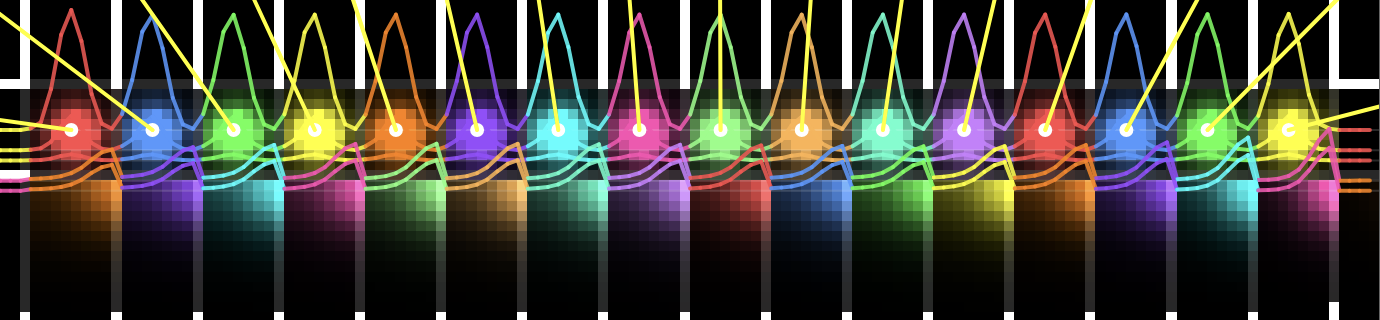
\includegraphics[width=\textwidth]{fig/cable_domains.png}
\caption{The cable, relaxed. Sixteen sites along the axis, each carrying a kernel of charge $+3$, a
core domain of two electrons confined within $c_r=2.4\,a_0$, and one valence electron outside it.
Colour distinguishes domains: the bright lobes on the axis are the cores, the fainter blocks beneath
them the valence charge standing off. White verticals mark the free boundaries between neighbouring
carriers, and the coloured curves are density profiles along a line through the axis; the yellow
segments are net forces on the kernels. The partition shown is the imposed one described in \S3 and
is held fixed while the wave functions relax, so the boundaries are inputs here rather than unknowns.
Displacing the middle $W$ of these carriers by half a spacing, at fixed cores and kernels, is the
quantity computed in \S3.}
\label{fig:cable}
\end{figure}

\paragraph{The standoff is set, not found.} The radius $c_r$ separating cores from carriers is
prescribed. It belongs to the specification of the arrangement, alongside the spacing, the kernel
charge and the number of electrons per site, and the conduction question is put to the arrangement
so specified. Whether a minimisation free to move that interface would settle at the same radius is
not decided here: released, the calculation does not converge at whole-cell resolution, and the
boundary that fails to settle is the one between neighbouring cores rather than the core--carrier
radius itself. The cable is therefore a stated geometry whose conduction is computed, not a
configuration the functional produces of itself.

\section{What sets the pinning}

The barrier is not set by the strength of the ion lattice but by whether the carriers bunch into its
wells. A carrier distribution that resisted being modulated would ride over the lattice; one that
does not resist locks to it.

RealQM's free interface resists very little, and this is internal to the construction. A flat density
is admissible on a free boundary at no cost --- a constant $\psi_i$ satisfies the normalisation, has
$\grad\psi_i=0$, and minimises the electrostatic energy against a neutralising background --- so
redrawing an interface between domains of equal density costs nothing. The partition therefore offers
no resistance to uniform compression, and the only penalty on a \emph{modulated} density is the
gradient term in \eqref{eq:E}, carrying the coefficient $\half$.

\paragraph{Sensitivity to the kinetic coefficient.} The kinetic term of \eqref{eq:E} carries the
nominal coefficient $\half$, and the question here is simply how much the barrier turns on it. What
follows is a sensitivity, not a calibration. No value was sought that would reproduce a conductivity, a barrier
or any other quantity taken from experiment, and none of the numbers below was known in advance.
The coefficient is varied from its physical $\half$ upward, with the ions, the standoff, the
geometry and the mesh unchanged:

\begin{center}
\small
\begin{tabular}{@{}lrrrrr@{}}
\toprule
coefficient $c$ & $0.50$ & $0.60$ & $0.75$ & $0.90$ & $1.00$\\
\midrule
$\varepsilon_{\rm bulk}$ (meV) & $246.1$ & $158.7$ & $66.4$ & $19.9$ & $1.0$\\
in units of $kT$ & $9.5$ & $6.1$ & $2.6$ & $0.77$ & $0.04$\\
\bottomrule
\end{tabular}
\end{center}

\noindent The preferred registry is the same at every point: the carriers sit on their own ion
sites throughout, so what falls is the pinning itself and not merely its location. The barrier
passes $kT$ between $c=0.75$ and $c=0.90$. A moderate stiffening of the carriers, well short of
the doubling, therefore brings this cable out of the range where charge is held and into the range
where thermal energy moves it.

The last entry should not be read as a value. One meV is a difference of $1.5\times10^{-4}$~Ha
between two total energies of $158$~Ha, below what this protocol has been shown to resolve. And the
entries away from $c=\half$ rest on the two ends $d=0$ and $d=\half$, so that the extrema lie there
remains an assumption for them --- an assumption that failed on the chain of \S4, whose minimum is
not at registry. It holds for the first entry, which has been scanned: that landscape is monotone
from registry to half-spacing, so its endpoints are its extrema and its $246$~meV is an amplitude.
Whether stiffening moves the extrema has not been tested.

\begin{center}
\small
\begin{tabular}{@{}lrl@{}}
\toprule
arrangement & barrier per carrier & preferred registry\\
\midrule
chain of H atoms & $394$~meV & off registry, near $d=\tfrac14$\\
cable of Li ions, carrier standing off & $246$~meV & carrier on its site\\
\quad the same cable at $c=0.9$ & $20$~meV & carrier on its site\\
\bottomrule
\end{tabular}
\end{center}

\paragraph{A transport number the landscape settles by itself.} A uniform field $F$ adds $-NeFd$ to the
energy: it tilts the landscape and changes nothing else. The field at which the barrier disappears
is therefore a property of $E(d)$ alone. No clock, no temperature and no dissipation enter it,
which is why it can be stated here, among the computed quantities, rather than in \S7 with the
conductivities. For
a sinusoid of amplitude $V_0$ the steepest slope is $\pi V_0/a$, so $F_{\rm th}=\pi V_0/ea$:
\begin{center}
\small
\begin{tabular}{@{}lrr@{}}
\toprule
arrangement & $V_0$ & $F_{\rm th}$ (V\,m$^{-1}$)\\
\midrule
chain of H atoms & $394$~meV & $5.2\times10^{9}$\\
cable of Li ions & $246$~meV & $3.2\times10^{9}$\\
\quad the same cable at $c=0.9$ & $20$~meV & $2.6\times10^{8}$\\
\bottomrule
\end{tabular}
\end{center}
\noindent Above that field charge advances without thermal help; below it, it does not advance at
all without. The three divide, and the division is the point. The first two are several times above the
dielectric strength of silica, ${\sim}10^{9}$~V\,m$^{-1}$, so those arrangements would break down
before they would slide --- which is what an insulator does. The stiffened cable is a factor of four
below it, so that one would slide first. The same separation that \S6 states as a barrier against
$kT$ appears here as a field against a breakdown strength, and neither statement needs a rate
theory to make it. The sinusoid enters here
as it does in $K$, and a scan of $E(d)$ at small $d$ would remove it, the threshold then following
from the computed slope directly. What does \emph{not} enter is any rate theory.

It is worth saying why the calculation stops at the threshold rather than continuing past it, since
driving the system further is the obvious thing to try. Below the threshold a local minimum
survives, so the pattern displaces a little and stops: that is an elastic response, the
polarisability of \S4, and no charge is transferred. Above it there is no minimum left and nothing
to stop the slide, so the field does work indefinitely and, in a conservative functional, that
energy has nowhere to go. There is no steady state to compute, and therefore no drift velocity.
The trap is that the solver will answer anyway. Driven past the threshold the partition does run and
walls do advance, so a speed can be read off --- but the relaxation is gradient descent in imaginary
time and its rate is the descent parameter, chosen rather than derived. The threshold is a property
of $E(d)$ and survives refinement; a current past it is a property of the scheme and does not.
Nothing in this article is computed above the threshold.

\section{What this gives, and what it does not}

In the activated regime the corrugation is the activation energy, and the conductivity of a hopping
conductor is
\begin{equation}\label{eq:sigma}
\sigma = \frac{n e^2 a^2 \nu}{kT}\,e^{-E_a/kT},
\qquad
\nu = \frac{1}{2\pi}\sqrt{\frac{K}{M}},
\end{equation}
with $\sigma$ the conductivity, $n$ the carrier density, $e$ the elementary charge, $a$ the hop
distance, $E_a$ the activation energy, $k$ Boltzmann's constant, $T$ the temperature, $\nu$ the
attempt frequency, $K$ the curvature of the well the carrier sits in and $M$ the mass of whatever
oscillates in it.

\paragraph{Activated rate theory.} The picture behind \eqref{eq:sigma} is Arrhenius's, made
quantitative \cite{hanggi}. A system sits in a potential well separated from the next by a barrier
$E_a$. It does not cross steadily. It oscillates in the well at the small-oscillation frequency set
by the curvature of the well and the mass in it, and on each oscillation there is some chance that
thermal fluctuation has put enough energy into the right coordinate for it to get over. The rate is
therefore a product of how often it tries and how often a try succeeds: $\nu$ counts the attempts,
and $e^{-E_a/kT}$ is the fraction of the time the Boltzmann distribution holds at least $E_a$ there.

The theory carries three conditions, and two of them will matter below. The barrier must be large
against $kT$: if it is not, crossings are not rare, the system spends a substantial part of its time
above the top, and the rate is set by how fast it moves rather than by how seldom it is lucky --- so
the factorisation into attempts and successes stops describing anything. The system must lose
the memory of one attempt before making the next, which in a solid it does by exchanging energy with
the lattice. And the barrier must be crossed over rather than through: $e^{-E_a/kT}$ is a classical
occupancy and says nothing about tunnelling.

That last one deserves an answer rather than an assumption, since tunnelling is often what carries
charge and the carriers here are electrons. The answer turns on which coordinate crosses. It is not
an electron moving through a barrier in space; it is the carrier pattern moving against the ion
lattice, and \S6 argues that the mass belonging to that motion is ionic, since it is the sites that
move. A coordinate that heavy tunnels feebly. Quantitatively, the crossover below which tunnelling
overtakes activation is $T_c=\hbar\omega_b/2\pi k$, which for the frequencies found here is
$179$~K for the chain and $43$~K for the cable. Both lie below room temperature, so the classical
factor is the right one at $300$~K --- though the chain is close enough to its crossover that
quantum corrections would not be negligible in a cold measurement. The argument is tied to the rigid
slide: a kink is a lighter object, and whether it tunnels is a question this article does not
reach.

What oscillates here is the collective coordinate $u$: the displacement of the carrier pattern along
the chain, the same variable $E(u)$ is evaluated against in \S3. The attempt is therefore the charge
pattern rocking back and forth in one corrugation well against the ion lattice, and since it is the
sites that move, that rocking is a lattice vibration. Both $V_0$ and $M$ are then taken per carrier,
which is consistent: displacing $m$ carriers rigidly costs $m$ times the barrier and moves $m$ times
the mass, and $\nu$ is unchanged.

RealQM supplies $E_a$, which decides the temperature dependence and the ratio between arrangements. The prefactor needs $K$, $M$ and $n$, and it is worth being exact about where each comes
from.

$K$ is the curvature of the landscape at its minimum, and it is the one place where the shape of
that landscape matters rather than its amplitude. Taking the periodic curve to be
$E(u)=\half V_0\bigl[1-\cos(2\pi u/a)\bigr]$ gives $K=2\pi^2V_0/a^2$, which for $V_0=246$~meV at
$a=4.5\,a_0$ is $0.80$~eV\,\AA$^{-2}$, and that is the value used below.

The scan of \S3 shows the assumption to be wrong, and in a direction worth stating. Across the half
period the cable gives, per carrier and relative to registry,
\begin{center}
\small
\begin{tabular}{@{}lrrrrr@{}}
\toprule
$d$ & $0$ & $0.125$ & $0.25$ & $0.375$ & $0.5$\\
\midrule
measured (meV) & $0$ & $-5$ & $+82$ & $+184$ & $+246$\\
sinusoid (meV) & $0$ & $+36$ & $+123$ & $+210$ & $+246$\\
\bottomrule
\end{tabular}
\end{center}
\noindent The landscape is monotone from registry to half-spacing, so the amplitude is the
difference of its endpoints after all and $V_0=246$~meV stands as a measured quantity rather than an
assumed one. But the curve lies below the sinusoid at every interior point, most of all near the
minimum, where it is flat out to $d=0.125$ instead of rising by $36$~meV. The well is therefore much
shallower in curvature than a sinusoid of the same amplitude, and since $\nu\propto\sqrt{K}$ the
attempt frequency below is an \emph{over}estimate and the conductivities with it. The steepest slope
runs the other way, $6\%$ above the sinusoidal value, so the threshold field is slightly
\emph{under}stated.

No corrected $K$ is quoted, because the interior points converge an order of magnitude less well
than the endpoints --- residuals of $0.04$ to $0.08$ against $0.004$ --- and a second difference over
a spacing of $0.125$ amplifies exactly that. What the scan establishes is the amplitude, and a
direction for the prefactor: the flatter the true minimum, the lower $\nu$ and the lower $\sigma$.

There is a second assumption in the same expression, of a different kind, and it should be stated
because no scan can remove it. Writing $\nu=\frac{1}{2\pi}\sqrt{K/M}$ is transition-state theory,
and transition-state theory describes one damping regime out of three. Kramers' result is that the
prefactor depends on the coupling $\gamma$ between the moving coordinate and the lattice, and
non-monotonically: strongly damped it becomes $\omega_0\omega_b/2\pi\gamma$, the rate being set by
how slowly the coordinate diffuses over the top; very weakly damped it is limited instead by how
slowly energy arrives. Only at intermediate damping does $\gamma$ cancel and the well curvature
alone set the rate. That intermediate case is the one assumed here, and it is assumed for a reason
worth admitting plainly: it is the only regime whose prefactor can be had from a landscape and a set
of masses. The other two require the coupling, which is the same quantity the driven regime needs
and which a functional without a boundary velocity cannot supply. One consequence runs against the
grain of the rest of this section --- transition-state theory \emph{over}estimates a rate, so this
prefactor biases $\sigma$ upward where the upper-bound barrier biases it down. The exponent wins by
orders of magnitude and the conductivities remain lower bounds, but the two errors do not point the
same way.

$M$ is part of the specification of the system rather than a parameter of the theory. Two masses
must be kept apart here. The \emph{electron} mass is genuinely absent from \eqref{eq:E}: the
coefficient of $|\grad\psi_i|^2$ is a geometric scale, not $\hbar^2/2m$, which is why \S6 can vary
it and why $E_a$ comes out without any mass being supplied. The \emph{nuclear} mass is a different
kind of thing --- a property of the nuclei one has chosen to put in the box. To say the material is
lithium is already to say $Z=3$ and $M=7\,u$, exactly as fixing the nuclear positions says what the
lattice is. It is needed only when the question turns from what the energy is to how fast something
oscillates in it. What moves here is the site, since the charge does not pass between sites but the
pattern of domains advances through the lattice, so $M$ is a nuclear mass and $\nu$ comes out a
lattice frequency.

$n=1/a^3$ is a convention for reporting rather than a quantity of either kind. It takes the cable's
spacing to hold in three dimensions, one carrier per site. The cable is a
single line of sites, so this is a stated convention for converting a per-carrier barrier into a bulk
conductivity, not something the calculation contains.

With the nuclear mass of the moving species --- $1\,u$ for the hydrogen chain, $7\,u$ for the
Li cable --- and $T=300$~K:

\begin{center}
\small
\begin{tabular}{@{}lrrrl@{}}
\toprule
 & $E_a$ & $\nu$ (Hz) & $\sigma$ (S/m) & for scale\\
\midrule
chain of H atoms & $394$~meV & $1.8\times10^{13}$ & $1.1\times10^{-1}$ & intrinsic Ge, $2$\\
cable of Li ions & $246$~meV & $5.5\times10^{12}$ & $10$ & intrinsic Ge, $2$\\
\quad the same cable at $c=0.9$ & $20$~meV & --- & --- & --- see below\\
\bottomrule
\end{tabular}
\end{center}

\noindent The attempt frequencies are $10^{12}$--$10^{13}$~Hz, which is where lattice vibrations
live: as an energy $h\nu$, $23$~meV for the cable and $97$~meV for the hydrogen chain, the latter high because a proton
is light. Nothing was arranged to make that so, and it is the check that the mass entering $\nu$ is
the right kind of mass. The first two rows bracket the conductivity of ordinary semiconducting
material, two orders of magnitude apart on a barrier ratio of $1.6$ --- the exponential at work,
since a difference of $148$~meV is $5.7\,kT$.

The third row carries no numbers because it violates the first condition above. At $E_a=20$~meV
against $kT=25.9$~meV the barrier is $0.77\,kT$ and $e^{-E_a/kT}=0.46$: the carriers are over the
top about half the time, so escape is not a rare event, $\nu$ counts nothing, and there is no sense
in which \eqref{eq:sigma} describes the state. Evaluating it there would
return a large conductivity, but the number would be an artifact of applying a rate law where no
rate is defined. What that state is, and what law governs it, this calculation does not determine.

These are order-of-magnitude statements and cannot be more. The $\pm30$~meV on $E_a$ is already a
factor $3.2$ either way in $\sigma$ at room temperature, the sinusoid is an assumption, and $M$ and
$n$ are inputs. What the framework delivers is the exponent; that the resulting numbers land in the
three named regimes, in the right order, with nothing fitted, is the result.

\paragraph{What a conductivity requires that a barrier does not.} The division of labour here is the
ordinary one. An energy landscape is computed from a theory of charge; a rate is then obtained from
it by a theory of statistics laid on top. Density functional theory with harmonic transition-state
theory does exactly this for diffusion and catalysis, and nobody regards the second step as a defect
of the first. What is unusual in this article is not the import but what sits underneath it: a
barrier with nothing fitted in it. It is still worth being exact about the distance between the two,
because the barrier is computed and the conductivity is not. Three things must be supplied, and
they are of three different kinds.

A \emph{clock}. A barrier says how high, a rate says how often, and the difference is an inertia.
The kinetic coefficient in \eqref{eq:E} is a geometric scale rather than $\hbar^2/2m$, so the
electronic functional carries no mass and can set no frequency. This one the framework can
nevertheless supply, because the nuclei do move classically: $\nu$ is a period read off a
trajectory rather than a curvature assumed, which is what \S8 records as now reachable.

A \emph{temperature}. Equation \eqref{eq:E} has no $T$ in it, no bath and nothing stochastic. The
entire apparatus of attempts and escapes, and the factor $e^{-E_a/kT}$ with it, is imported from
activated rate theory and laid over a static minimisation. The model can neither confirm it nor
refute it, and this is the largest single import in \S6.

A \emph{dissipation channel} --- but only in the other regime, and the distinction is worth keeping
straight. Below threshold the bath that supplies a fluctuation also takes the energy back between
hops, which is why the system returns to a minimum each time and why nothing accumulates; dissipation
is implicit in the temperature and needs no separate account. Above threshold there is no barrier to
be activated over, $T$ drops out, and dissipation must instead be explicit, or a carrier merely
accelerates and there is no steady drift at all. That regime is not treated here. Its ingredients are
not absent in principle --- the nuclei are classical, so the electron--lattice channel other
treatments import is present in the equations and $\tau$ would be an output rather than an input ---
but nothing of the kind is computed.

So the regime this article works in needs two imports, not three: a frequency and a temperature.
With those, the drift velocity follows from the landscape directly,
$v_d = (ea^2\nu F/kT)\,e^{-E_a/kT}$ at small field, every other quantity in it being computed ---
the barrier, the hop distance, and the density of sites.

Of these, only the temperature is an import in the strong sense --- a statistics the framework
does not contain and cannot check. The other two are provisional rather than structural: the clock
because the nuclei are already dynamical, the dissipation because those same nuclei are the channel
through which a carrier would lose its energy. So the present arrangement, a computed landscape with
a rate theory brought in from outside, is the expected first stage rather than the end of the matter,
and what would replace it is stated in \S\ref{sec:further}.

\paragraph{The kink, and why the table is a lower bound.} Every barrier above is a rigid slide: all
carriers displaced together, so the cost is $N$ times a per-carrier barrier --- which the windowed
measurement establishes rather than assumes, the linearity in $W$ having been tested against a third
window --- and the whole sample must climb at once. Real conductors do not do this, and no
macroscopic sample could.

What a cheaper path saves is not the total work. Both routes run between the same two
configurations, which on a wrapped chain are equivalent minima, so each is a climb to a saddle and
a return; and moving the same charge the same distance costs at least as much summed along a
sequential path as along a simultaneous one. What differs is the height of the saddle --- the
largest energy that must be present at a single instant --- because that is what a thermal
fluctuation has to supply in one go, and it is therefore what sets the rate. A sample requiring
$N\varepsilon$ at once is quiet for ever at any $N$ of physical size; one requiring $\varepsilon$ at
a time, $N$ times, is not. The mechanical analogue is a carpet, which is dragged whole only against
the friction of its whole area but is moved a ruck at a time for less force and, if anything, more
total work.

That alone makes the table an upper bound, and by an argument that does not depend on knowing what
the sample does instead. The barrier is the minimum, over all paths joining one registry to the
next, of the greatest energy along the path; the rigid slide is one such path; a minimum over a set
is at most its value at any member. So the numbers above bound the activation energy from above
whatever the mechanism turns out to be, and the conductivities bound it from below.

What the cheaper path \emph{is} is not settled here. The carriers on their substrate are a
Frenkel--Kontorova chain \cite{braun}, whose standard cheap path is a kink --- a localised
compression or rarefaction of the carrier lattice, moving by shifting its centre --- and \S8 sets
out what computing one would require. Until it is computed the gap between the rigid slide and the
true barrier is not determined, and neither is the factor by which every $\sigma$ above is an
underestimate. That is the principal limitation of the numbers in this section, and it is worth
being plain that it is not a small one: $\sigma$ depends exponentially on the barrier, so the
agreement in the table with intrinsic silicon and germanium is contingent on the bound being
reasonably tight, which nothing here establishes.

One consequence is worth recording because it follows from the construction rather than from the
kink picture. Doping cannot mean here what it usually means: there is no band to add a carrier to
and no gap to promote one across. What can be added is a \emph{domain}, and since the domains tile,
an added domain takes its space from its neighbours and compresses the carrier lattice locally while
a removed one lets them expand. So $n$- and $p$-type would be compression and rarefaction, the
dopant concentration would set the density of these defects, and conduction would proceed by moving
the very defects that doping creates --- with an $n/p$ asymmetry that is structural rather than
fitted. None of it is computed, and a dopant at a realistic concentration is one atom in $10^3$,
which sixteen sites cannot represent.

What is outside is not a regime but a kind of quantity. A resistive conductivity
$\sigma=ne^2\tau/m$ needs a momentum relaxation time from electron--phonon scattering, and that needs
a current as an object, electron dynamics, and irreversibility; a minimisation over real densities
has none of the three, at any barrier height. And band conduction specifically is absent in kind
rather than by degree: non-overlap admits no extended states, so there is nothing for a band to be
made of, and no choice of stiffness produces one. Neither of these tells us what the unpinned state
of \S5 is. They say only that if it conducts, it does not do so by filling bands, and that this
framework will not supply the rate at which it does.

\section{A first three-dimensional lattice, and further studies}\label{sec:further}

The nuclei of \S4 and \S5 lie on a line. The calculation does not: it is three-dimensional
throughout, and what is restricted is the lattice, not the electronic problem. A line is the
smallest arrangement in which the question can be posed, and it is why $n=1/a^3$ is a convention
there rather than a count. The obvious
next step is real configurations in three dimensions: the tetrahedral lattice of silicon and
germanium, the close-packed lattices of the alkali metals, the layered structures of the oxides.
Nothing in \eqref{eq:E} is one-dimensional, and the angular splitting of a kernel's valence sector
already reaches the bonding topologies these lattices are built from. A three-dimensional cell would
make the carrier density a property of the structure rather than a stated convention, and would let
a barrier be compared with the activation energy of a named material instead of with a range.

\paragraph{A first three-dimensional lattice.} That step has been taken for the simplest case, and
it is worth reporting both for what it settles and for what it does not. Hydrogen has no core and no
standoff, so unlike the cable there is no lower bound on how close neighbouring chains may sit ---
the cable needs $c_{\rm sep}\gtrsim1.6\,a$, its cores occupying $2c_r$ and its carriers needing room
between them --- and hydrogen atoms can therefore be placed on a simple cubic lattice at the same
spacing $a$ in all three directions. Seventy-two of them, $3\times3\times8$ at $a=4.5\,a_0$, one
electron per kernel and nothing imposed beyond the lattice itself.

\begin{figure}[htb]
\centering
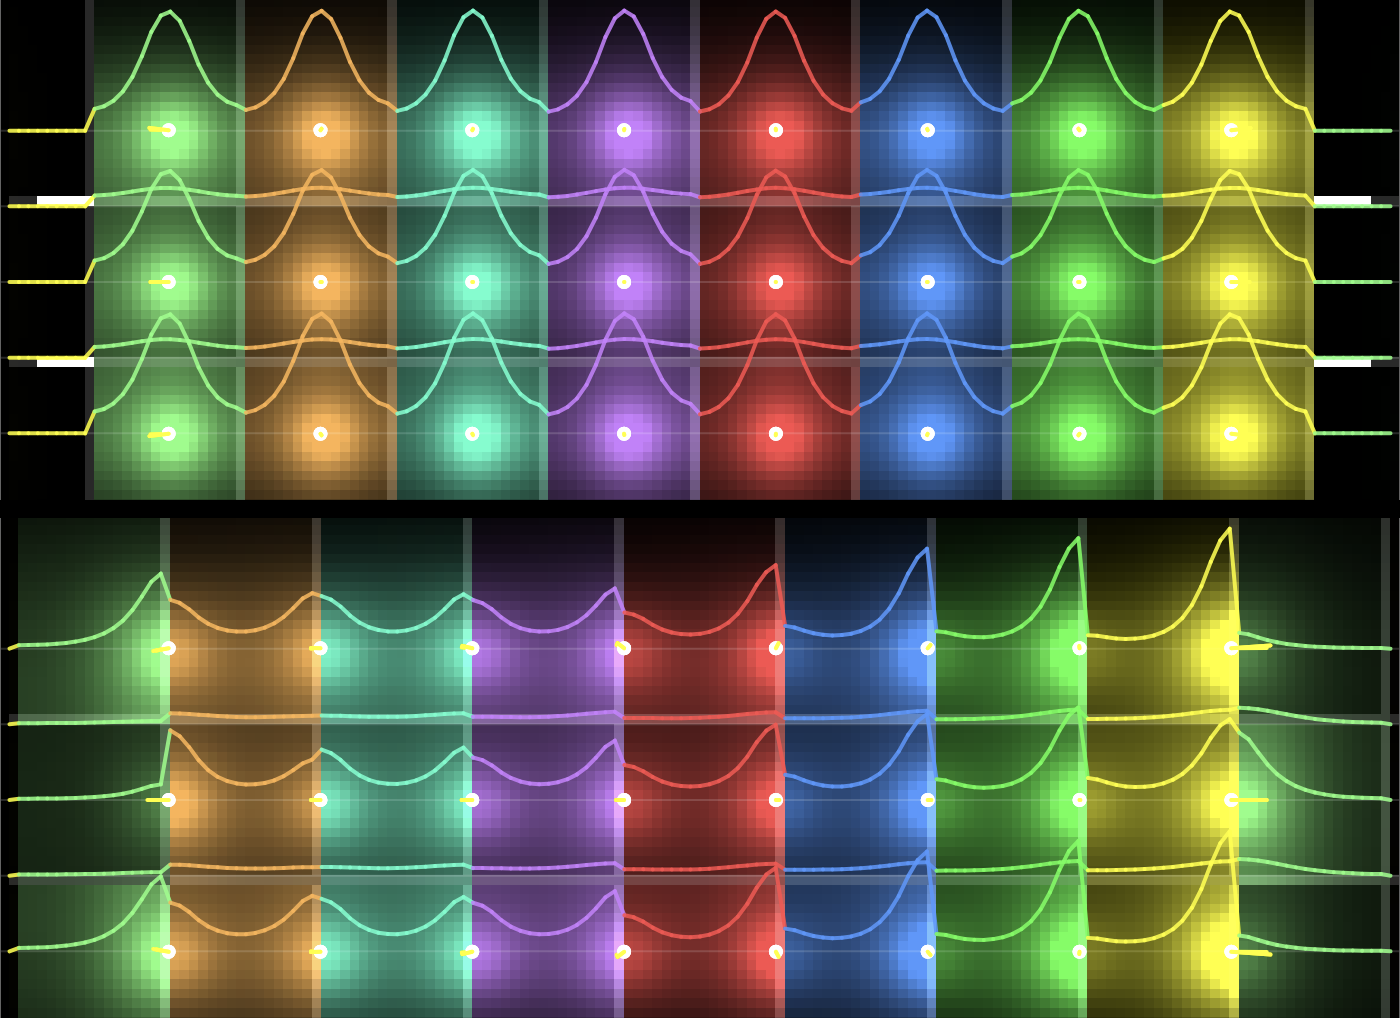
\includegraphics[width=\textwidth]{fig/hlat_pair.png}
\caption{Simple cubic hydrogen, $3\times3\times8$ at $a=4.5\,a_0$, in its two registries. The frame
is a plane through the lattice at fixed $z$, so three of the nine chains appear, eight sites each,
one electron per kernel and no core, no cutoff and no standoff anywhere in the construction. White
dots are the protons, colour distinguishes domains, the white verticals are the boundaries between
neighbouring electrons along a chain, and the curves are density profiles along each chain.
\emph{Above}, $d=0$: every domain is centred on its own proton and each profile is a single peak on
the nucleus. \emph{Below}, $d=\half$: the boundaries now sit on the protons, so each domain spans
from one nucleus to the next and its electron is shared between the two bounding it --- the profiles
go double-humped and the charge piles against the walls. The two differ in nothing but where the
boundaries sit, and the energy between them is the quantity this article computes. Both are at the
same step count, since two states relaxed to different degrees would not be comparable. Note also
that the boundaries run through all three chains at the same $x$, which is what makes $d$ one
collective coordinate for the whole lattice rather than one per chain.}
\label{fig:hlat}
\end{figure}

The construction is verified three ways. At $1\times1$ it reproduces, to all nine digits, an
eight-site chain at the finer mesh --- not the sixteen-site chain of \S4, which is a different
system; the comparisons in this section are all against that eight-site one, and are marked as
such. The nuclear sum over the $72$ protons agrees with an independent evaluation of the same
lattice to eleven figures. And the translation control holds exactly: at a matched step count
$E(d{=}1)$ and $E(d{=}0)$ agree to every digit reported, which they must, a displacement of one full
spacing being a relabelling of the same calculation.

What it settles is the binding. The lattice gives $-0.524$~Ha per atom against that eight-site
chain's $-0.453$ --- a gap of $1930$~meV per atom, against which the clamp's failure to cancel
between two different arrangements is of order $80$ --- and below even the exact free atom's $-0.5$, because a domain in the lattice is a
compact cell of volume $a^3$ rather than a slab running out to the box face. It is also the
better-conditioned calculation, which was not expected of nine times the domains: its residual at
$d=0$ is $5.3\times10^{-4}$, against $1.8\times10^{-3}$ for that chain and $4\times10^{-3}$ for the cable, the
smallest in this article. A partition into compact cells is evidently closer to what the functional
would choose than one into elongated slabs, and $n=1/a^3$ is exact for this arrangement where \S6
must state it as a convention.

What it does not settle is the barrier, and the record is worth giving in full rather than
summarising. The two ends do not relax at the same rate here, where the chain's two ends agree
within a factor of two:

\begin{center}
\small
\begin{tabular}{@{}rrrr@{}}
\toprule
steps & residual at $d=0$ & residual at $d=\half$ & $[E(\half)-E(0)]/N$\\
\midrule
$2000$ & $5.4\times10^{-4}$ & $5.9\times10^{-2}$ & $739$~meV\\
$4000$ & $5.3\times10^{-4}$ & $1.1\times10^{-2}$ & $650$~meV\\
$8000$ & $5.3\times10^{-4}$ & $1.7\times10^{-3}$ & $678$~meV\\
\bottomrule
\end{tabular}
\end{center}

\noindent The last column is not a barrier and is not labelled as one: it is the global difference
between two displacements, unwindowed, so it carries the junctions. It is given to show that the
quantity does not settle. The unslid end is converged --- it moves by $0.007$~meV per electron over the last
doubling. The slid end is not, moving by $28$, although its residual falls steadily by a factor of
six or seven each time. And the barrier itself is not monotone, so it cannot be extrapolated:
$E(\half)$ descends and then rises again, where the same ladder on the cable rose throughout. A
fixed-partition relaxation that steps an energy down and then up is not something this article can
account for, and until it can, the $4000$-step point is better read as an excursion than as a stage.

\paragraph{The windowed measurement, and why the global difference is withdrawn.} The windowing of
\S3 has since been applied to the lattice, and it does not correct the global difference above --- it
contradicts it. The window displaces the middle $W$ sites of all nine chains together, so $d$ remains
one collective coordinate and each window costs $9W$ bulk plus eighteen junctions; differencing $W=2$
against $W=4$ gives $\varepsilon_{\rm bulk}=[E(4)-E(2)]/18$ as before. The port was gated first: at
$\mathtt{hlat=1x1}$ with the window disabled it reproduces the global slide to nine digits.
\begin{center}
\small
\begin{tabular}{@{}rrrrr@{}}
\toprule
$d$ & $E(W{=}2)$ (Ha) & $E(W{=}4)$ (Ha) & residual & $\varepsilon_{\rm bulk}$ (meV)\\
\midrule
$0.125$ & $-37.918398$ & $-38.091914$ & $5.4\times10^{-4}$ & $-262$\\
$0.250$ & $-38.311165$ & $-38.894297$ & $5.5\times10^{-4}$ & $-882$\\
$0.375$ & $-38.363507$ & $-39.022777$ & $5.9\times10^{-4}$ & $-997$\\
$0.500$ & $-36.980096$ & $-36.375537$ & $2.4\times10^{-3}$ & $(+914)$\\
\bottomrule
\end{tabular}
\end{center}
\noindent The first three are converged to the standard of the best measurements in this article.
The fourth is not: its residual is four times worse and it is the configuration whose domain walls
sit \emph{on} the protons --- the end the ladder above already identifies as the one that will not
relax --- so it is bracketed and not used.

What the three converged points show is that \textbf{registry is not the minimum of this lattice}.
The landscape descends away from it, monotonically over the range measured, reaching $997$~meV per
carrier below registry at $d=\tfrac38$. The global difference of $678$~meV is therefore
\emph{withdrawn} rather than qualified. It is not an overestimate of a barrier: it is a difference
between two configurations neither of which is an extremum, which is precisely the error the chain's
scan exposed in \S4 and which \S3 warns against in its own words. The forty per cent the chain's
ends contributed is not the relevant correction here; the ends were not inflating a barrier, they
were producing one.

The amplitude is not supplied in its place. Half the period rests on the unconverged $d=\half$
point, the scan has not been repeated at a second mesh, and the minimum has not been bracketed
beyond $d=\tfrac38$. What the lattice establishes is therefore structural --- that the construction
is verified three ways, that the binding per atom rises from $-0.453$ to $-0.524$~Ha on going from a
line to a crystal, that $n=1/a^3$ is exact for it, and that its preferred registry is not the one
assumed --- and not a barrier.

The scale needed for this is not out of reach, and that is the practical consequence of the cost
being linear in $N$ rather than exponential, as \S1 establishes. The solids already computed in this
framework, listed there and reaching a hundred atoms \cite{code}, were asked structural and thermal
questions; what has not been attempted in any of them is transport. It is also what several of
the questions below require rather than merely benefit from. A dopant at a realistic concentration
is one atom in $10^3$ or fewer, so doping cannot be represented on sixteen sites at all --- the
account of $n$- and $p$-type in \S7 needs a cell large enough to hold one dopant and the lattice
around it. The same is true of a kink, whose width is set by the ratio of two curvatures and which
must fit inside the cell with bulk on either side of it, and of grain boundaries, interfaces and
vacancies, which are where the transport of real material is usually decided.

The one quantity still owed can be discharged two ways. A scan of $E(d)$ at small $d$ gives the
curvature directly and retires the assumed sinusoid. Better, moving the nuclei under their classical
equations of motion --- which the framework does, and which is the one genuine clock in it, the
relaxation iteration being imaginary time --- gives the attempt frequency as a period read off a
trajectory, making both the curvature and the assumed shape unnecessary.

The kink is the larger prize. Every barrier here is a rigid slide, so every barrier is an upper
bound and every conductivity a lower bound by a factor this article does not determine. Measuring
the formation energy $E_f$ and the Peierls--Nabarro barrier $E_{\rm PN}$ would replace bounds with
values, and would at the same time make the account of doping in \S7 testable: $n$- and $p$-type as
compression and rarefaction of the carrier lattice, dopant concentration setting the kink density,
and an $n/p$ asymmetry that is structural rather than fitted.

One defect in the discretisation blocks more than any single calculation. Positions live on the
grid, so a displacement smaller than a cell does not exist, and at the mesh used here one cell is an
eighth of a spacing. The defect has two halves. One of them has since been repaired, which is worth
reporting because it changes what is owed and what is merely not yet done.

Nuclear coordinates were truncated to whole cells when handed to the solver, and are now carried as
continuous ones. Two quantities return with them. The attempt frequency can be obtained as it was
meant to be --- by releasing the kernels and reading a period off a trajectory, which retires the
assumed curvature altogether --- since a thermal oscillation of some $0.3\,a_0$ at room temperature
is no longer rounded away. And the Peierls instability of a conjugated chain, the distortion that
makes polyacetylene a semiconductor and gives its solitons something to be a defect in, is about
$0.03\,a_0$ per carbon or a sixth of a cell: a chain that previously returned identical energies at
five values of the distortion now resolves them. Neither quantity is computed in this article.
Both are now reachable, which they were not.

The other half stands, and four quantities wait on it --- all of them a boundary moving rather than
a nucleus. A domain wall still sits in one cell or the next. The polarisability must therefore be
computed with the partition frozen, since a released boundary answers a sub-threshold field by
moving zero cells or one. A boundary driven at fixed force either sticks or chatters between
adjacent cells, so a depinning threshold cannot be read. The Peierls--Nabarro barrier needs a kink
profile finer than a cell. And $\kappa$, the second Frenkel--Kontorova constant, requires a
non-uniform displacement small enough to be harmonic --- smaller than the grid can express, so
amplitudes below a cell return the undisplaced chain exactly. Carrying the boundary as a volume
fraction rather than by whole-cell ownership would release all four, and is the single change the
programme of this section most depends on.

That constant is worth naming as an aim in its own right. The chain of carriers on a periodic
substrate is a Frenkel--Kontorova system \cite{braun}, the standard phenomenological account of
commensurate lattices, depinning and kink transport, and its two constants are the substrate
amplitude and the coupling. RealQM computes the first: $V_0$ is the corrugation computed here, which
in ordinary use is supplied from data. With the second, the same model yields the kink width, the
Peierls--Nabarro barrier and the Aubry pinning criterion \cite{aubry} with nothing further put in.
The transport would then be done by a model whose credentials are not in question, from constants
this framework computed rather than fitted --- which is a sharper claim than a conductivity resting
on an assumed curvature. It is worth noting which standard models are \emph{not} available in the
same way: a Hubbard or tight-binding description is degenerate here, since non-overlap makes the
transfer integral vanish identically, and Frenkel--Kontorova fits because its degrees of freedom are
the ones RealQM has.

Two questions are open in a way that could change the account rather than sharpen it. Whether RealQM
has a self-consistent standoff --- a cable whose core--carrier radius the functional settles at
rather than one supplied with the specification --- is the first, and \S5 records that it cannot be
decided at this resolution, the released calculation being the one place where whole-cell interfaces
bite hardest. The
second is whether the arrangement in which the barrier all but vanishes conducts in any useful
sense, or is merely an unpinned lattice that still holds its charge per site; the polarisability
scaling is the test,
since charge fixed per site gives $\alpha\propto N$ whatever the barrier.

Finally, and to state the contact with measurement at its proper strength. No computed number here
is set against a measured number for the same system, because these arrangements have no
experimental counterpart. What can be said is that three quantities of different kinds land in the
ranges measurement gives, none of them arranged to: barriers of $246$--$394$~meV where semiconductor
activation is measured at $50$--$500$; attempt frequencies at $h\nu=23$ and $97$~meV, which are
lattice-vibration energies, and would have come out two orders higher had the mass been the
electron's --- though computed from a sinusoid's curvature, which \S6 shows to be too sharp, so the
frequencies themselves are overestimates even as their scale is right; and threshold fields several times above the dielectric strength of silica, so that these
arrangements would fail before they would slide, as insulators do. That is consistency in magnitude
across three independent quantities from a calculation with nothing fitted in it. It is not a test,
and it should not be read as one.

A test needs a system that has been measured. The sharpest available is not a value but a slope:
the activation energy fixes the temperature dependence of $\sigma$, and an Arrhenius plot of a real
activated conductor measures the same quantity directly. A conjugated chain such as polyacetylene is
the natural candidate --- a real material, measured activation energies, transport by the localised
defects \S7 describes, and doping in the sense described above --- and \S\ref{sec:further} records
what remains before it can be computed.

\section{Conclusion}

For a chain of hydrogen atoms, one electron to each kernel, RealQM gives a barrier of $394$~meV per
electron for the electron pattern to advance one site, and a polarisability $\alpha=7.6N$, extensive
in the number of electrons. Its landscape is not the assumed one: the minimum lies near a quarter
spacing rather than at registry, so the arrangement in which each electron is centred on its own
kernel is not the one the functional prefers.

For a cable of Li ions with the carriers standing off closed cores it gives $246$~meV, a factor of
$1.6$ less. The two cannot be built from the same ion, and the reason is instructive: a carrier can
stand off a core only if there is a core, and since the domains tile, one domain per kernel must
contain its kernel --- so a standoff requires at least two electrons per site where the chain has
one. The difference in ion is entailed by the difference in arrangement rather than chosen alongside
it. What is the same is the physics: \eqref{eq:E} throughout, with nothing fitted in either.

Stiffening the carriers of that cable lowers the barrier steeply and without changing the preferred
registry: at a coefficient of $0.9$ against the nominal $\half$, it is $20$~meV, below room temperature's
$kT$, and the charge is no longer held. So the barrier is set
less by the ion lattice than by how strongly the carrier distribution resists being modulated by it,
which is a property of the interface condition rather than of the interaction.

Placing the same atoms on a simple cubic lattice rather than a line settles the binding and not
the barrier. Seventy-two hydrogen atoms, $3\times3\times8$, give $-0.524$~Ha per atom against the
eight-site chain's $-0.453$ and below even the exact free atom's $-0.5$, because a domain in the
lattice is a compact cell rather than a slab running out to the box face; $n=1/a^3$ is exact for it
where \S6 must state it as a convention. It yields no barrier: windowed and scanned, its landscape
descends away from registry, by $997$~meV per carrier at a three-eighths displacement, so registry is
not its minimum either. The chain's minimum lies off registry in one dimension and the lattice's does
in three.

What the lattice also shows is where the cost of this method lies, since it bears on how far the
calculation can be taken. Nine times the domains did not make the problem harder: at $d=0$ the
lattice's residual is $5.3\times10^{-4}$, against $1.8\times10^{-3}$ for the eight-site chain at
the same mesh and $4\times10^{-3}$ for the cable, the smallest in this article, a partition into compact cells being
evidently closer to what the functional would choose. The work is the one of \S1 --- $N$ Poisson solves on a single
grid --- so atoms enter the count once each. At the mesh used here, $h=0.281\,a_0$, a $200^3$ grid spans $56\,a_0$ and holds
of order a thousand atoms at this spacing, which is within the memory of a single consumer GPU, though
such a run would take days rather than the hour and a half the lattice took. A
system of that size is therefore a question of time and of memory, not of a different method. What it is not is quick, and the cost divides in a way worth stating. A single relaxation step is
cheap --- about $0.25$~s on the $138^3$ box and $0.6$~s on the $148^3$ lattice, so the eight-thousand
step runs above take an hour and a half each, and a $200^3$ grid would be some two and a half times
that per step. What is expensive is the number of steps the \emph{difference} requires. The energy
settles long before the barrier does: on the cable a $200$-step run is already stable to look at and
is $5.7$~Ha from its converged value, and on the lattice the ladder of \S8 still moves the
\emph{difference} between $4000$ and $8000$ steps while $E(0)$ has stopped changing in the sixth
figure. Shortening the
relaxation is therefore not a dial that trades accuracy for time smoothly; it is what the step ladders
are for. The limit on this calculation is patience and the constraints it has to impose, not dimension.

Taking each barrier as an activation energy and closing the prefactor with an attempt frequency
built from the same landscape and a nuclear mass puts the first two arrangements at $10^{-1}$ and
$10^{1}$~S\,m$^{-1}$, bracketing intrinsic germanium, with the attempt frequencies coming out at
lattice values unasked --- a check that the mass in them is of the right kind, though the
frequencies themselves are overestimates, being built on a curvature the scan shows to be too
sharp. Nothing in this is fitted. What the calculation takes beyond \eqref{eq:E} is a specification
of the system --- which nuclei, at what spacing, under what geometric constraint --- together with a
convention for reporting a bulk density, and a theory of rates to turn an energy into a current. The conductivities are lower bounds, the rigid slide being one path between the two registries
and the barrier the minimum over all of them; by how much is not determined here, since the cheaper
path has not been computed. What the framework does not deliver in any regime
is a resistive conductivity, whose relaxation time needs a current as an object and irreversible
dynamics: a minimisation over real densities has neither.

\appendix
\section{Computational details}\label{sec:details}

All calculations use the RealQM solver \texttt{molecule.js} driven by \texttt{chain\_slide.html}
(WebGPU, single GPU). Equation \eqref{eq:E} is minimised by imaginary-time relaxation of the
densities on a uniform Cartesian grid, with the partition specified by a cell-ownership map.

\paragraph{The code, and running it.} Everything is at
\begin{center}\small\url{https://github.com/Claes542/RealMolecule}\end{center}
and runs \emph{in a web browser} with nothing to install, compile or configure: the solver is
JavaScript and WGSL, the arithmetic is done by WebGPU on whatever GPU the machine has, and a run is
started by opening a page. A WebGPU-capable browser is required --- Chrome or Edge at present. Every
configuration in this article is a query string, so each calculation below is reproduced by following
one link. The reference state and the two windows that give the $246$~meV of \S5:
\begin{center}\small
\url{https://claes542.github.io/RealMolecule/chain_slide.html?n=16&a=4.5&rc=0&rsing=1.5&cps=8&wrap=1&coax=1&kq=3&ncore=2&chom=1&cr=2.4&steps=4000&d=0}
\end{center}
and the same with \texttt{\&swin=4\&d=0.5} and \texttt{\&swin=8\&d=0.5}, which are the pair the
barrier is differenced from; the stiffened runs of \S6 add \texttt{\&kins=$c$} together with a step
count scaled in proportion to $c$, for the reason given below. Each run stops at the step count in
its own query string and then writes its total energy, its Euler--Lagrange residual and its
per-domain eigenvalues into
\texttt{localStorage} under \texttt{realqm\_resid}, keyed by the full configuration, so the numbers in
the tables below are read out rather than transcribed from the screen. The parameters are named in
the source at the top of \texttt{chain\_slide.html}. For
every corrugation the partition is \emph{frozen}: the energy of a stated configuration is evaluated,
which is legitimate for configurations related by a symmetry of the lattice and is why translation by
one spacing is used as the control. Energies are reported in hartree and converted at
$1$~Ha${}=27211$~meV.

\paragraph{The chain of hydrogen atoms.} $N=16$ atoms in a row at $a=4.5\,a_0$, nuclear charge
$+1$, one electron per site, no pseudopotential. Wrapped labelling, so translation by one spacing is
an exact relabelling. Mesh $8$ cells per spacing, box $=(N-1)a+10=77.5\,a_0$, grid $138^3$,
$h=0.5616\,a_0$; nuclear cutoff $r_{\rm sing}=0.6\,a_0$. Fixed $4000$ steps. Windowed at $W=4$ and
$W=8$, so the two junctions cancel in the difference and
$\varepsilon_{\rm bulk}=[E(8)-E(4)]/4$ is the bulk cost per electron, relative to registry:
\begin{center}
\small
\begin{tabular}{@{}rrrr@{}}
\toprule
$d$ & $E(W{=}4)$ (Ha) & $E(W{=}8)$ (Ha) & $\varepsilon_{\rm bulk}$ (meV)\\
\midrule
$0.125$ & $-5.358520213$ & $-5.372141768$ & $-92.7$ \\
$0.250$ & $-5.372645480$ & $-5.401376734$ & $-195.5$ \\
$0.375$ & $-5.353253672$ & $-5.347920417$ & $+36.3$ \\
$0.500$ & $-5.273676889$ & $-5.244451806$ & $+198.8$ \\
\bottomrule
\end{tabular}
\end{center}
\noindent The displacements available are multiples of $a/8$: domain boundaries are whole-cell, so
half a cell is not representable and such a run does not converge. Amplitude $394$~meV per electron,
minimum near $d=\tfrac14$, maxima of $0$ and $+199$~meV.

The cutoff dependence was measured separately, on an eight-site chain at the finer mesh of $16$
cells per spacing: $E(0)=-3.623964481$ and $E(\half)=-3.435219214$ at $r_{\rm sing}=0.6\,a_0$
against $E(0)=-3.394494680$ and $E(\half)=-3.217398798$ at $0.8\,a_0$, so the totals move by
$0.2295$~Ha $=6.24$~eV while their difference moves by $39.6$~meV, a suppression of $158$.

Polarisability from the induced dipole at $F=5\times10^{-4}$~au with the partition
frozen, at $N=4,6,8$: $\alpha/N = 7.55,\ 7.63,\ 7.70\,a_0^3$. The dipole is taken as the
difference between the field-on and field-off runs, which removes a small common offset.

\paragraph{The cable of Li ions.} $N=16$ sites at $a=4.5\,a_0$ on the
axis, kernel charge $+3$, one core domain per site carrying two electrons and confined within
$c_r=2.4\,a_0$ of the axis, one valence electron per site outside that radius: $32$ domains, neutral,
and no pseudopotential, so the carrier is excluded from the core region by non-overlap alone. Mesh $8$ cells per spacing, box $=(N-1)a+10=77.5\,a_0$, grid $138^3$,
$h=77.5/138=0.5616\,a_0$; the box is the chain span plus a fixed pad and so does not depend on the
mesh. Only differences between the two registries of this system are used; its total energy is not.
Only the shell slides; the cores and kernels are held. All runs use the fixed-step protocol below,
at $r_{\rm sing}=1.5\,a_0$ (above $2h=1.123$). Windowed energies at $d=\half$, $W$ the number of
displaced carriers:
\begin{center}
\small
\begin{tabular}{@{}lrr@{}}
\toprule
 & $W=4$ & $W=8$\\
\midrule
$E$ (Ha), $4000$ steps & $-149.542323$ & $-149.506148$\\
\bottomrule
\end{tabular}
\end{center}
\noindent Equation \eqref{eq:window} then gives $\varepsilon_{\rm bulk}=246.1$~meV per carrier.

\paragraph{The nuclear cutoff, and a correction.} A bare $-Z/r$ well cannot be represented on a
grid, so it is clamped at a radius $R_{\rm sing}$. The solver sets
$R_{\rm sing}=\max(2h,\,r_{\rm sing})$ with $r_{\rm sing}$ a requested absolute value, and the
requested $0.5\,a_0$ used here is smaller than $2h$ at every mesh employed --- $1.12$, $0.90$ and
$0.75\,a_0$ at $8$, $10$ and $12$ cells per spacing. The cutoff was therefore $2h$ throughout, tied
to the grid rather than absolute, and refining the mesh sharpens the ion instead of merely resolving
it. An earlier version of this appendix stated that the clamp fixed the potential as the same object
at every mesh; that is not what the code does, and any comparison across meshes made under that
assumption compares different ions rather than one ion at different resolutions. To hold the
potential fixed, $r_{\rm sing}$ must be set above $2h$ at the finest mesh in use.

What the cutoff costs, and where it cancels, is worth recording since it is the largest numerical
error here. On a hydrogen atom at $r_{\rm sing}=0.6$ it is $89$~mHa, or $2.4$~eV --- more than any
barrier in this article. It cancels between two configurations of one system at one cutoff, which is
what a corrugation is: changing it from $0.6$ to $0.8\,a_0$ moves the chain's total by $6.2$~eV and
its barrier by $40$~meV. It does \emph{not} cancel between different systems. Over a cutoff interval
of $0.26\,a_0$ the chain moves $123$~meV per atom against the free atom's $46$, the chain electron
being pressed toward its nucleus by its neighbours and so carrying more density inside the cutoff.
Nor can the cutoff simply be shrunk: it is bounded below by $2h$, so reducing it means refining the
grid, and at the smallest value reachable here the chain comes out more bound per atom than the
exact H$_2$ molecule, the cutoff by then spanning some two cells. Every energy difference quoted in
this article is therefore taken at one cutoff between configurations of one system; no binding
energy is quoted against experiment or against another method's number, and none could be without
treating the nuclear cusp analytically rather than truncating it. The two per-atom bindings compared
in \S8 are RealQM values at one mesh and one cutoff, and the clamp does not cancel exactly between
them, the two arrangements being different: the scale of that residue is the $123$ against
$46$~meV per atom quoted just above, against a gap of $1930$.
\paragraph{Stiffened carriers.} Identical geometry, mesh and ion lattice, with the coefficient of
$|\grad\psi_i|^2$ raised from $\half$ to $1$ for the shell domains only, the cores keeping $\half$.
The coefficient enters three places --- the imaginary-time step, the $H\psi$ diagnostic and the
energy sum --- and all three must carry it or the reported energy does not belong to the state
produced. The explicit step requires the diffusion number below $1/6$, so the timestep is halved in
proportion, and the stiffened runs are given $8000$ steps rather than $4000$ to cover the same
relaxation. The coefficient is set by \texttt{\&kins=}$c$ and was run at
$c=0.50,\ 0.60,\ 0.75,\ 0.90$ and $1.00$, giving the sensitivity tabulated in \S6. The value the
body quotes is the one at $c=0.90$, $\varepsilon_{\rm bulk}=19.9$~meV, which is resolved. At the
doubling, $c=1.00$, the windowed pair is $E(W{=}4)=-157.965427$ and $E(W{=}8)=-157.965275$~Ha and
\eqref{eq:window} returns $1.04$~meV; that is $1.5\times10^{-4}$~Ha out of $158$, below what this
protocol resolves, and it is reported here only to complete the record.

\paragraph{The cubic lattice.} $72$ hydrogen atoms, $3\times3\times8$ at $a=4.5\,a_0$ in all three
directions, nuclear charge $+1$, one electron per site, no core, no standoff and no pseudopotential.
Mesh $16$ cells per spacing, $h=0.28125\,a_0$; box $=(8-1)a+10=41.5\,a_0$, grid $148^3$. The
requested cutoff $r_{\rm sing}=0.6\,a_0$ exceeds $2h=0.5625\,a_0$ at this mesh, so here --- unlike
the $138^3$ runs discussed above --- the cutoff is the absolute one and not the grid-tied value.
Wrapped along the chain direction; $d$ displaces all nine chains together at the same $x$, so it is
one collective coordinate:
\begin{center}\small\url{https://claes542.github.io/RealMolecule/chain_slide.html?n=8&a=4.5&rc=0&rsing=0.6&cps=16&wrap=1&hlat=3x3&hsep=4.5&steps=8000}\end{center}
At $4000$ steps $E(0)=-37.742193495$ with residual $5.3\times10^{-4}$ and
$E(\half)=-36.023663034$ with residual $1.1\times10^{-2}$. The step ladder is given in full in \S8
and does not settle, which is why no barrier is quoted for this system; the windowing of \S3 is
\emph{not} applied here, so the difference between the two displacements carries the junctions as
well as the bulk. Controls: $E(d{=}1)=E(d{=}0)=-37.742193495$ to every digit, a displacement by one
full spacing being a relabelling; the nuclear sum over the $72$ protons agrees with an independent
evaluation to eleven figures; and at $\mathtt{hlat=1x1}$ the construction reproduces the eight-site
chain at the same mesh to nine digits. Runs at $8000$ steps take several hours each on a single
consumer GPU.

\paragraph{The windowed lattice.} The same $72$-atom lattice with the window of \S3 applied along
the chain direction, so the middle $W$ sites of all nine chains displace together and $d$ stays one
collective coordinate:
\begin{center}\small\url{https://claes542.github.io/RealMolecule/chain_slide.html?n=8&a=4.5&rc=0&rsing=0.6&cps=16&wrap=1&hlat=3x3&hsep=4.5&swin=2&d=0.250&steps=2000}\end{center}
and the same with \texttt{\&swin=4}, which is the pair the $d=0.250$ entry is differenced from;
the other displacements substitute \texttt{\&d=0.125}, \texttt{0.375}, \texttt{0.500}. Each window
costs $9W$ bulk plus eighteen junctions, so
$\varepsilon_{\rm bulk}=[E(W{=}4)-E(W{=}2)]/18$. Fixed $2000$ steps: the step ladder of \S8 is for the
unwindowed slide, and the windowed states are far better conditioned than it --- $5.4\times10^{-4}$
at $2000$ steps against $1.1\times10^{-2}$ for the unwindowed slid end at $4000$. That is not
incidental. Windowing makes the displaced state a local perturbation of the undisplaced one rather
than a global rearrangement, which is why the unwindowed ladder would not settle.
The port was gated before any of it was run: at \texttt{\&hlat=1x1\&swin=0} the windowed code
reproduces the eight-site chain at $-3.623964481$, to nine digits, which is the value the unwindowed
branch returns.

\paragraph{The fixed-step protocol.} Runs are stopped after a stated number of relaxation steps
rather than when the energy stops changing. The energy test --- three consecutive frames within
$2\times10^{-5}$~Ha --- halts at a different step count for every configuration, so two windowed
energies would be relaxed to different degrees and their difference, which is the quantity wanted, would
mix the two; and a configuration that never satisfies it runs to the step cap, which is weeks.
A fixed count makes each run reproducible from its URL, the solver being deterministic to nine
digits, and makes the windowed difference a comparison of like with like. Calibration on the cable
at $c_r=2.4$, $W=4$: $E=-155.354541$ at $200$ steps, $-150.281715$ at $1000$, $-149.615172$ at
$2000$, $-149.542323$ at $4000$, $-149.542140$ at $8000$. Four thousand steps is used throughout;
eight thousand moves the energy by $5.0$~meV. The Euler--Lagrange residual plateaus at
$4.0\times10^{-3}$ from $2000$ steps onward --- $0.0233$, $0.0059$, $0.00404$, $0.00403$, $0.00403$
along the same ladder --- while at $2000$ steps the energy is still $1.98$~eV from its $4000$-step
value, so the residual detects gross non-convergence but cannot be the sole test.

This ladder also sets the scale against which the stiffening of \S6 must be read. A single total
energy still moves $5$~meV between $4000$ and $8000$ steps. The windowed difference removes what the
two configurations have in common, and both are run to the same step count, so most of that drift is
common to them; but no test here bounds the remainder below a few meV. The value \S6 quotes,
$19.9$~meV at $c=0.90$, stands clear of that scale by a factor of four. The $1.04$~meV at the
doubling does not, which is the second reason --- alongside its being $1.5\times10^{-4}$~Ha out of
$158$ --- that it is reported as a record rather than as a barrier.

\paragraph{The rate estimate of \S6.} Equation \eqref{eq:sigma} evaluated at $T=300$~K
($kT=25.9$~meV) with $a=4.5\,a_0=2.381$~\AA, $n=1/a^3=7.4\times10^{28}$~m$^{-3}$, the nuclear mass of the moving species, and
$K=2\pi^2V_0/a^2$ from the assumed sinusoid, giving $\nu=(1/a)\sqrt{V_0/2M}$:
\begin{center}
\small
\begin{tabular}{@{}lrrrrr@{}}
\toprule
$V_0$ (meV) & $K$ (eV\,\AA$^{-2}$) & $\nu$ (Hz) & $\sigma_0$ (S/m) & $e^{-V_0/kT}$ & $\sigma$ (S/m)\\
\midrule
$1000$ & $3.48$ & $5.5\times10^{12}$ & $1.4\times10^{5}$ & $1.6\times10^{-17}$ & $2.3\times10^{-12}$\\
$240$ & $0.84$ & $2.7\times10^{12}$ & $7.0\times10^{4}$ & $9.3\times10^{-5}$ & $6.5$\\
$24$ & $0.084$ & $8.5\times10^{11}$ & $2.2\times10^{4}$ & $0.395$ & $8.8\times10^{3}$\\
\bottomrule
\end{tabular}
\end{center}
\noindent Taking $M=m_e$ instead of an ionic mass raises $\nu$ to $6.1\times10^{14}$~Hz and $\sigma$
to $1.5\times10^{3}$~S\,m$^{-1}$ on the middle row; that frequency is two orders above any lattice
vibration, which is the argument for the ionic choice quite apart from the physical one. The $\pm30$
meV uncertainty on the middle row is a factor $3.2$ in $\sigma$.

\paragraph{Convergence and resolution.} The states entering each windowed difference are relaxed
but not fully converged, carrying Euler--Lagrange residuals of $2\times10^{-3}$ for the chain of
\S4 and $4\times10^{-3}$ for the cable of \S5; the stiffened runs halve the timestep for stability
and are less relaxed than the others. Every number
reported is for the stated system at the stated mesh, with the nuclear cutoff held at an absolute
radius above $2h$ so that it belongs to the model rather than to the grid. Whether the same numbers
survive a different discretisation, or a different implementation of the same equations, is not
established here and is left to further work.

\paragraph{Controls applied.} Translation by one full period must return the same energy: satisfied
to nine digits ($E(0)=E(N)$ exactly) on the wrapped geometries. Repeat runs of one configuration
agree to nine digits, so the solver is deterministic and any discrepancy is attributable to the
model or the input. Domains related by a symmetry must have equal eigenvalues: this is what exposed
the terminal domains of a finite cable binding an electron-volt harder than the interior, and hence
the necessity of \eqref{eq:window}.

\section*{On the use of computational assistance}

The solver and the drivers used here were written with AI assistance, and the analysis was carried
out the same way. Two statements make that disclosure precise, and the second is what licenses the
first.

No quantity in the model is calibrated to any measurement. \eqref{eq:E} contains Coulomb
interaction and kinetic energy and nothing else; what the calculation takes beyond it is a
specification of the system --- which nuclei, at what spacing, under what geometric constraint ---
and a stated convention for reporting a bulk density. Nothing was adjusted to reproduce a barrier, a
conductivity or any other number, and none of the values reported was known in advance of computing
it.

The implementation is checkable against standards independent of it, and was checked. A hydrogen
atom must come out at $-0.5$~Ha; two separated unit charges must repel as $1/R$; translation of a
wrapped chain by one spacing is a relabelling and must return the same energy, which it does to nine
digits; repeat runs of one configuration must agree, and do, to the last reported digit. That
discipline is not a formality. It found, in the course of this work, that the nuclear cutoff was
tied to the mesh rather than fixed, so that refining the grid sharpened the ion instead of resolving
it; and that nuclear coordinates are truncated to whole cells before the solver sees them, which is
why several quantities named in \S\ref{sec:further} cannot presently be computed at all. Neither is a fitted
parameter, and both changed what the calculation means.

The distinction worth drawing is therefore not between assistance with code and assistance with
physics, which would suppose that implementation is innocent --- it is not, as those two findings
show. It is between content calibrated to the data it is meant to explain, which absorbs
disagreement, and content derived from a stated principle, which is exposed to it. This article
contains none of the first kind.

\begin{thebibliography}{99}
\bibitem{ashcroft} N.~W. Ashcroft and N.~D. Mermin, \emph{Solid State Physics}, Holt, Rinehart and
Winston, New York, 1976.
\bibitem{kohnsham} W.~Kohn and L.~J. Sham, Self-consistent equations including exchange and
correlation effects, \emph{Phys. Rev.} \textbf{140}, A1133 (1965).
\bibitem{perdewlevy} J.~P. Perdew and M.~Levy, Physical content of the exact Kohn--Sham orbital
energies: band gaps and derivative discontinuities, \emph{Phys. Rev. Lett.} \textbf{51}, 1884 (1983).
\bibitem{hedin} L.~Hedin, New method for calculating the one-particle Green's function with
application to the electron-gas problem, \emph{Phys. Rev.} \textbf{139}, A796 (1965).
\bibitem{bardeen} J.~Bardeen and W.~Shockley, Deformation potentials and mobilities in non-polar
crystals, \emph{Phys. Rev.} \textbf{80}, 72 (1950).
\bibitem{marcus} R.~A. Marcus, On the theory of oxidation--reduction reactions involving electron
transfer. I, \emph{J. Chem. Phys.} \textbf{24}, 966 (1956).
\bibitem{holstein} T.~Holstein, Studies of polaron motion: Part II. The ``small'' polaron,
\emph{Ann. Phys.} \textbf{8}, 343 (1959).
\bibitem{mott} N.~F. Mott, Conduction in non-crystalline materials III. Localized states in a
pseudogap and near extremities of conduction and valence bands, \emph{Philos. Mag.} \textbf{19}, 835
(1969).
\bibitem{hubbard} J.~Hubbard, Electron correlations in narrow energy bands, \emph{Proc. R. Soc.
London A} \textbf{276}, 238 (1963).
\bibitem{imada} M.~Imada, A.~Fujimori and Y.~Tokura, Metal--insulator transitions, \emph{Rev. Mod.
Phys.} \textbf{70}, 1039 (1998).
\bibitem{dm21} J.~Kirkpatrick \emph{et al.}, Pushing the frontiers of density functionals by
solving the fractional electron problem, \emph{Science} \textbf{374}, 1385 (2021).
\bibitem{mace} I.~Batatia, D.~P. Kov\'acs, G.~N.~C. Simm, C.~Ortner and G.~Cs\'anyi, MACE: higher
order equivariant message passing neural networks for fast and accurate force fields,
\emph{Adv. Neural Inf. Process. Syst.} \textbf{35}, 11423 (2022).
\bibitem{ferminet} D.~Pfau, J.~S. Spencer, A.~G.~D.~G. Matthews and W.~M.~C. Foulkes, Ab initio
solution of the many-electron Schr\"odinger equation with deep neural networks, \emph{Phys. Rev.
Research} \textbf{2}, 033429 (2020).
\bibitem{hanggi} P.~H\"anggi, P.~Talkner and M.~Borkovec, Reaction-rate theory: fifty years after
Kramers, \emph{Rev. Mod. Phys.} \textbf{62}, 251 (1990).
\bibitem{braun} O.~M. Braun and Y.~S. Kivshar, \emph{The Frenkel--Kontorova Model: Concepts, Methods,
and Applications}, Springer, Berlin, 2004.
\bibitem{aubry} S.~Aubry, The twist map, the extended Frenkel--Kontorova model and the devil's
staircase, \emph{Physica D} \textbf{7}, 240 (1983).
\bibitem{simons17} M.~Motta \emph{et al.} (Simons Collaboration on the Many-Electron Problem),
Towards the solution of the many-electron problem in real materials: equation of state of the
hydrogen chain with state-of-the-art many-body methods, \emph{Phys. Rev. X} \textbf{7}, 031059
(2017).
\bibitem{simons20} M.~Motta \emph{et al.} (Simons Collaboration on the Many-Electron Problem),
Ground-state properties of the hydrogen chain: dimerization, insulator-to-metal transition, and
magnetic phases, \emph{Phys. Rev. X} \textbf{10}, 031058 (2020).
\bibitem{realqm} C.~Johnson, \emph{Real Quantum Mechanics}, \url{https://realqm.com}.
\bibitem{code} C.~Johnson, \emph{RealMolecule}: RealQM solver and browser front-ends,
\url{https://github.com/Claes542/RealMolecule}. Runs in a WebGPU browser with no installation; the
gallery of live calculations is at \url{https://claes542.github.io/RealMolecule/gallery.html}.
\bibitem{realqmbook} C.~Johnson, \emph{Real Quantum Mechanics: a new view of the atom}, book
manuscript.
\bibitem{realatoms} C.~Johnson, \emph{A 3D multiphase continuum computational model for atoms},
manuscript; ionisation energies across the periodic table.
\bibitem{realnucleus} C.~Johnson, \emph{RealNucleus: nucleons as charge densities}, manuscript;
nuclear binding by dual Coulomb confinement.
\end{thebibliography}

\end{document}
